% ============================================================================
% STATISTICS
% ============================================================================

\section{Codebase Statistics}
\label{sec:statistics}

This section presents detailed statistics about the \ctx{} codebase.

\subsection{Overall Metrics}

\begin{table}[h]
\centering
\begin{tabular}{lr}
\toprule
\textbf{Metric} & \textbf{Value} \\
\midrule
Total Source Files & 20 \\
Total Lines of Code & $\approx$ 8,500 \\
Total Symbols & 548 \\
Total Edges (Relationships) & 2,664 \\
\bottomrule
\end{tabular}
\caption{Overall codebase metrics}
\label{tab:overall-metrics}
\end{table}

\subsection{Symbol Distribution}

\begin{table}[h]
\centering
\begin{tabular}{lrr}
\toprule
\textbf{Symbol Kind} & \textbf{Count} & \textbf{Percentage} \\
\midrule
Functions & 446 & 81.4\% \\
Structs & 35 & 6.4\% \\
Enums & 11 & 2.0\% \\
Traits & 3 & 0.5\% \\
Constants & 53 & 9.7\% \\
\midrule
\textbf{Total} & \textbf{548} & \textbf{100\%} \\
\bottomrule
\end{tabular}
\caption{Symbol distribution by kind}
\label{tab:symbol-distribution}
\end{table}

\subsection{Per-File Breakdown}

\begin{longtable}{lrrrr}
\toprule
\textbf{File} & \textbf{Total} & \textbf{Functions} & \textbf{Public} & \textbf{Types} \\
\midrule
\endhead
\file{main.rs} & 43 & 38 & 2 & 0 \\
\file{db/schema.rs} & 74 & 65 & 52 & 3 \\
\file{parser/mod.rs} & 40 & 32 & 28 & 4 \\
\file{formatter.rs} & 47 & 42 & 38 & 3 \\
\file{parser/typescript.rs} & 41 & 36 & 8 & 2 \\
\file{parser/python.rs} & 44 & 40 & 8 & 1 \\
\file{index/mod.rs} & 34 & 28 & 15 & 2 \\
\file{analytics/mod.rs} & 31 & 26 & 18 & 2 \\
\file{embeddings/mod.rs} & 29 & 24 & 18 & 3 \\
\file{parser/rust.rs} & 26 & 22 & 6 & 1 \\
\file{embeddings/openai.rs} & 25 & 22 & 4 & 1 \\
\file{parser/solidity.rs} & 22 & 19 & 5 & 1 \\
\file{embeddings/local.rs} & 21 & 18 & 4 & 1 \\
\file{db/models.rs} & 28 & 12 & 12 & 9 \\
\file{cli.rs} & 18 & 8 & 8 & 6 \\
\file{tree.rs} & 15 & 12 & 8 & 1 \\
\file{walker.rs} & 14 & 11 & 8 & 1 \\
\file{output.rs} & 10 & 8 & 6 & 1 \\
\file{default\_ignores.rs} & 3 & 2 & 2 & 0 \\
\bottomrule
\caption{Symbol count per file}
\label{tab:per-file}
\end{longtable}

\subsection{Edge Distribution}

\begin{table}[h]
\centering
\begin{tabular}{lrr}
\toprule
\textbf{Edge Kind} & \textbf{Count} & \textbf{Percentage} \\
\midrule
Calls & 2,412 & 90.5\% \\
Imports & 198 & 7.4\% \\
Extends & 32 & 1.2\% \\
Implements & 22 & 0.8\% \\
\midrule
\textbf{Total} & \textbf{2,664} & \textbf{100\%} \\
\bottomrule
\end{tabular}
\caption{Edge distribution by kind}
\label{tab:edge-distribution}
\end{table}

\subsection{Most Connected Functions}

Functions with the highest connectivity (combined fan-in and fan-out):

\begin{table}[h]
\centering
\begin{tabular}{lrrr}
\toprule
\textbf{Function} & \textbf{Fan-Out} & \textbf{Fan-In} & \textbf{Total} \\
\midrule
\func{extract\_symbols} (typescript) & 48 & 4 & 52 \\
\func{extract\_symbols} (solidity) & 48 & 4 & 52 \\
\func{discover\_files} & 46 & 2 & 48 \\
\func{parse\_response} & 45 & 1 & 46 \\
\func{parse} (typescript) & 20 & 43 & 63 \\
\func{extract\_symbols} (rust) & 42 & 3 & 45 \\
\func{watch\_and\_index} & 41 & 1 & 42 \\
\func{build\_signature} (typescript) & 39 & 2 & 41 \\
\func{extract\_call\_edges} & 37 & 4 & 41 \\
\func{run\_query} & 37 & 1 & 38 \\
\bottomrule
\end{tabular}
\caption{Most connected functions}
\label{tab:connected-functions}
\end{table}

\subsection{Code Quality Metrics}

\begin{table}[h]
\centering
\begin{tabular}{lr}
\toprule
\textbf{Quality Metric} & \textbf{Value} \\
\midrule
Functions analyzed & 446 \\
High complexity functions & 17 (3.8\%) \\
Critical complexity functions & 0 (0\%) \\
Duplicate code pairs (80\%+ similarity) & 13 \\
Average function fan-out & 6.0 \\
Median function fan-out & 4 \\
Maximum function fan-out & 48 \\
Functions with zero fan-out & 89 (20\%) \\
\bottomrule
\end{tabular}
\caption{Code quality metrics}
\label{tab:quality-metrics}
\end{table}

\subsection{Language Distribution}

All source files are written in Rust:

\begin{table}[h]
\centering
\begin{tabular}{lrr}
\toprule
\textbf{Language} & \textbf{Files} & \textbf{Percentage} \\
\midrule
Rust & 20 & 100\% \\
\bottomrule
\end{tabular}
\caption{Source file language distribution}
\label{tab:language-dist}
\end{table}

\subsection{Module Size Distribution}

\begin{figure}[h]
\centering
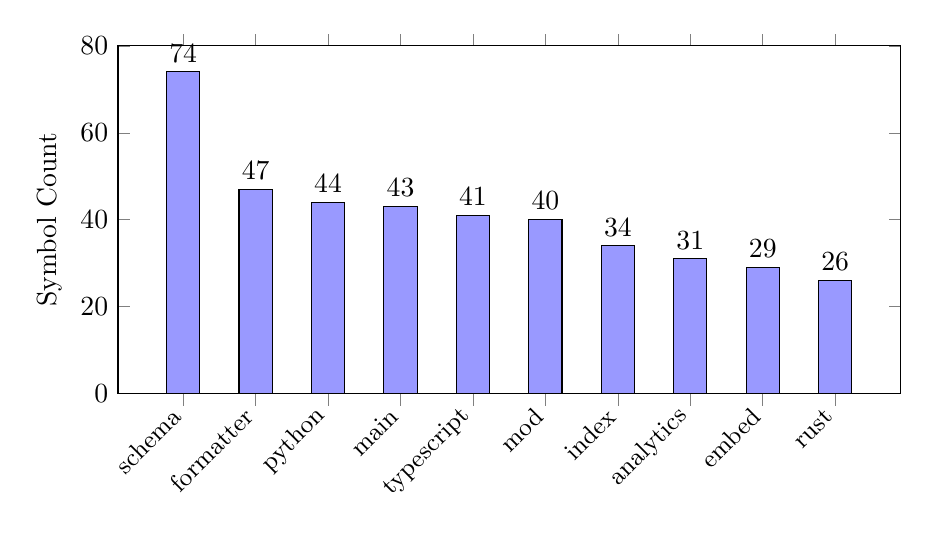
\begin{tikzpicture}
\begin{axis}[
    ybar,
    ylabel={Symbol Count},
    symbolic x coords={schema, formatter, python, main, typescript, mod, index, analytics, embed, rust},
    xtick=data,
    x tick label style={rotate=45, anchor=east, font=\small},
    ymin=0,
    ymax=80,
    bar width=12pt,
    nodes near coords,
    nodes near coords align={vertical},
    width=0.95\textwidth,
    height=6cm,
]
\addplot[fill=blue!40] coordinates {
    (schema, 74)
    (formatter, 47)
    (python, 44)
    (main, 43)
    (typescript, 41)
    (mod, 40)
    (index, 34)
    (analytics, 31)
    (embed, 29)
    (rust, 26)
};
\end{axis}
\end{tikzpicture}
\caption{Top 10 modules by symbol count}
\label{fig:module-size}
\end{figure}

\subsection{Test Coverage Areas}

The codebase includes tests for the following areas:

\begin{itemize}
    \item \textbf{Parser tests} --- Symbol extraction and call edge detection for each language
    \item \textbf{Formatter tests} --- Output format correctness
    \item \textbf{Database tests} --- CRUD operations and query correctness
    \item \textbf{Walker tests} --- File discovery and ignore patterns
    \item \textbf{Integration tests} --- End-to-end indexing workflows
\end{itemize}

\subsection{External Dependencies}

Key external crates used:

\begin{table}[h]
\centering
\begin{tabular}{ll}
\toprule
\textbf{Crate} & \textbf{Purpose} \\
\midrule
\code{clap} & Command-line argument parsing \\
\code{rusqlite} & SQLite database access \\
\code{duckdb} & Analytical queries \\
\code{tree-sitter} & Source code parsing \\
\code{tree-sitter-*} & Language-specific grammars \\
\code{ignore} & Gitignore-style file filtering \\
\code{fastembed} & Local embedding generation \\
\code{reqwest} & HTTP client for OpenAI API \\
\code{serde} & Serialization/deserialization \\
\code{flate2} & Gzip compression \\
\code{sha2} & Content hashing \\
\code{notify} & File system watching \\
\bottomrule
\end{tabular}
\caption{Key external dependencies}
\label{tab:dependencies}
\end{table}
